% ------------------------------------------------------------------------------
% TYPO3 Version 10 LTS - What's New (English Version)
%
% @author	Michael Schams <schams.net>
% @license	Creative Commons BY-NC-SA 3.0
% @link		https://typo3.org/help/documentation/whats-new/
% @language	English
% ------------------------------------------------------------------------------

\section{Dashboard}
\begin{frame}[fragile]
	\frametitle{Dashboard}

	\begin{center}\huge{\color{typo3darkgrey}\textbf{Dashboard}}\end{center}
	\begin{center}\large{\textit{Systeeminformatie, nieuws en meer voor backend-gebruikers}}\end{center}

\end{frame}

% ------------------------------------------------------------------------------
% Feature | 90333 | Dashboard

\begin{frame}[fragile]
	\frametitle{Dashboard}
	\framesubtitle{Backend-weergave}

	Een nieuw dashboard toont belangrijke informatie over het systeem aan de huidige backend gebruiker.

	\begin{figure}
		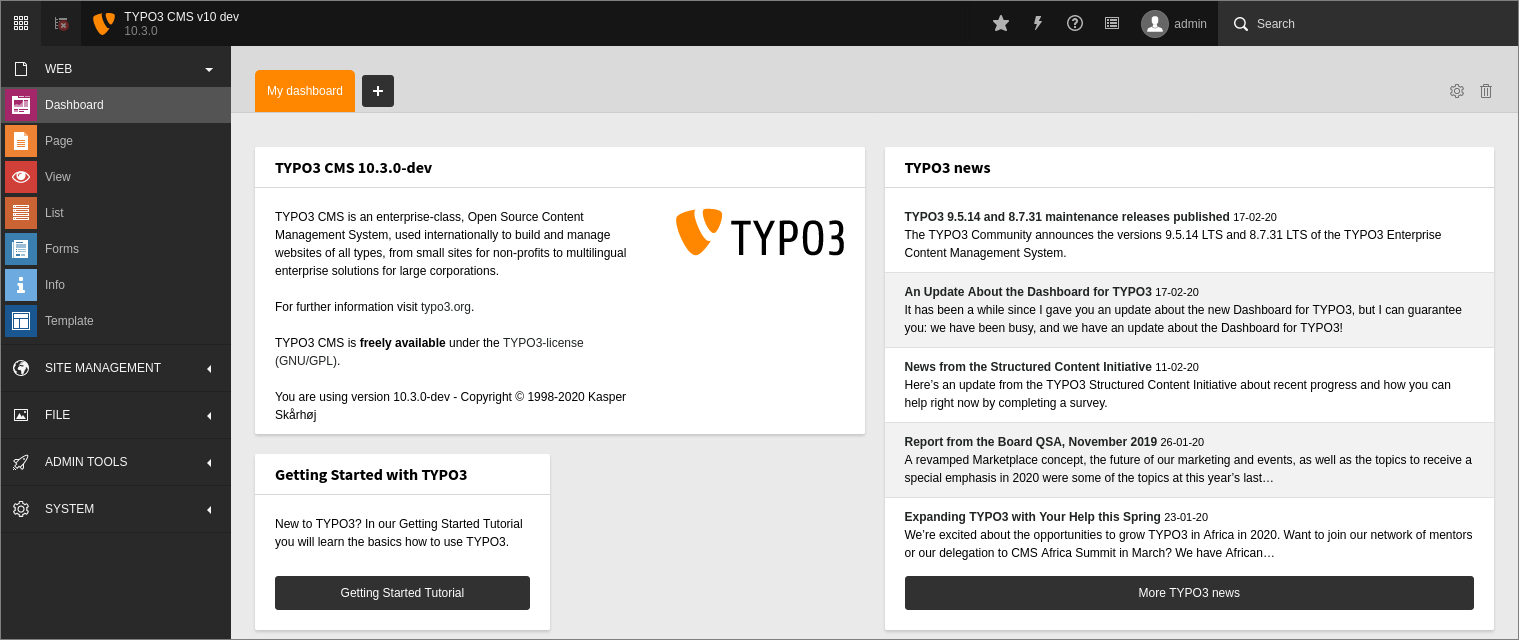
\includegraphics[width=0.9\linewidth]{Dashboard/90333a-Dashboard.png}
	\end{figure}

\end{frame}

% ------------------------------------------------------------------------------
% Feature | 90333 | Dashboard

\begin{frame}[fragile]
	\frametitle{Dashboard}
	\framesubtitle{Backend-weergave}

	Gebruikers kunnen hun eigen dashboards maken en "widgets" toevoegen, verwijderen en ordenen.

	\begin{figure}
		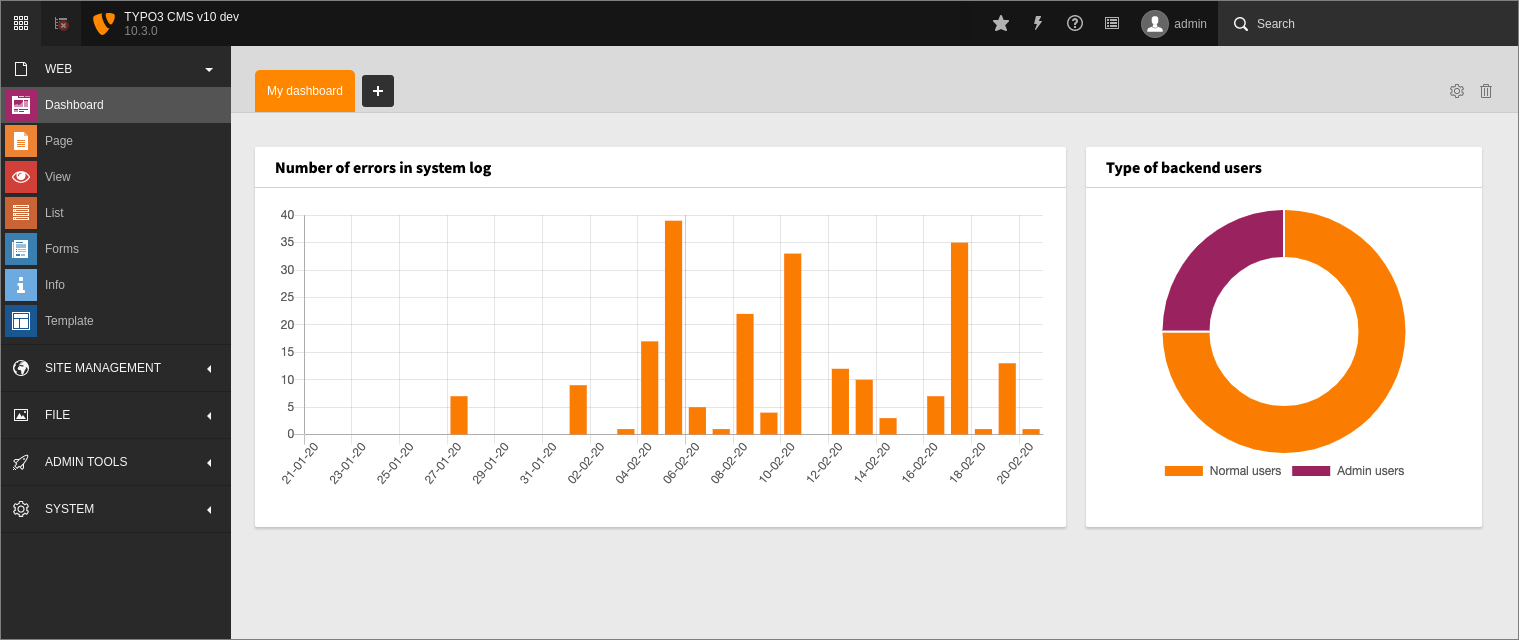
\includegraphics[width=0.9\linewidth]{Dashboard/90333b-Dashboard.png}
	\end{figure}

\end{frame}

% ------------------------------------------------------------------------------
% Feature | 90333 | Dashboard

\begin{frame}[fragile]
	\frametitle{Dashboard}
	\framesubtitle{Options for Integrators}

	% decrease font size for code listing
	\lstset{basicstyle=\tiny\ttfamily}

	\begin{itemize}
		\item Dashboard \textit{voorinstellingen} kunnen geconfigureerd worden voor nieuwe gebruikers of voor gebruikers
			die alle dashboards verwijderd hebben.
		\item Dit kan gebruikt worden om een "Snelstart" dashboard als standaard te tonen.
		\item Voorbeeld TSconfig:

\vspace{-0.4cm}
\begin{lstlisting}
options.dashboard.dashboardPresetsForNewUsers = default, dashboardPreset-myPreset
\end{lstlisting}

		\item Meerdere dashbooard-voorinstellingen kunnen gedefinieerd worden in een kommagescheiden lijst.
	\end{itemize}

\end{frame}

% ------------------------------------------------------------------------------
% Feature | 90333 | Dashboard

\begin{frame}[fragile]
	\frametitle{Dashboard}
	\framesubtitle{Eigen Widgets}

	\begin{itemize}
		\item TYPO3 v10 LTS heeft standaard een aantal widgets\newline
			\smaller
				(bijvoorbeeld: algemene informatie, mislukte inlogpogingen backend, TYPO3 nieuws, links naar documentatie, etc.)
			\normalsize
		\item Ontwikkelaars kunnen eigen widgets bouwen als extensies.
		\item Registreer en configureer widgets in een YAML bestand:\newline
			\small
				\texttt{EXT:myextension/Configuration/Services.yaml}
			\normalsize
		\item De systeemextensie "Dashboard" biedt een aantal typische widgets\newline
			\smaller
				(staafdiagram, "actie"-knop, donut-grafiek, lijst, getal met icoon en rss widget)
			\normalsize
		\item Meer over het dashboard in de
			\href{https://docs.typo3.org/c/typo3/cms-dashboard/master/en-us/}{TYPO3 documentatie}.

	\end{itemize}

\end{frame}

% ------------------------------------------------------------------------------
